\documentclass[crop,tikz]{standalone}% 'crop' is the default for v1.0, before it was 'preview'
\usepackage{tikz,calc,pgfplots}
\usepackage{tikz-3dplot}
\usetikzlibrary{calc}
\usetikzlibrary{calc,patterns,decorations.pathmorphing,decorations.markings}
\usetikzlibrary{shapes.geometric}
\begin{document}

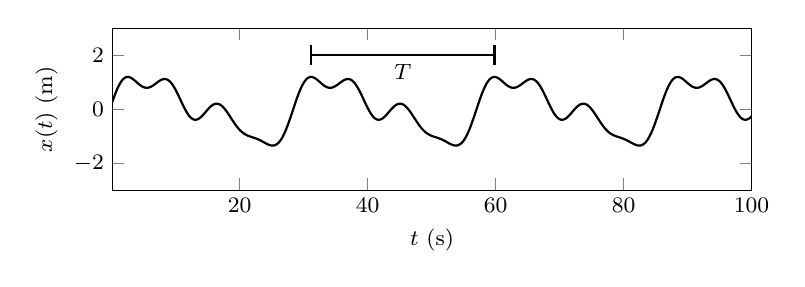
\begin{tikzpicture}[scale=1]
	\footnotesize
	\begin{axis}[
		width=0.8\textwidth,
		height=0.3\textwidth,
		xlabel={$t$ (s)},
		ylabel = {$x(t)$ (m)},
		xmax=100,
		xmin=0.1,
		ymax=3,
		ymin=-3,
		samples=500,
		ylabel near ticks]
		
		
		\def\wn{2*2*pi};
				
		\addplot[black, thick, domain=0.1:100] (x, {sin(\wn * x) + 0.5* sin(2*\wn * x) + 0.2*cos(3*\wn * x) + 0.3*sin(4*\wn * x)});
		
		\draw [|-|, thick] (axis cs: 31,2) -- (axis cs: 60,2) node [pos=0.5,below] {$T$};
		
	\end{axis}
	
\end{tikzpicture}

\end{document}